%!TEX TS-program = xelatex
\documentclass[]{friggeri-cv}
\usepackage{afterpage}
\usepackage{hyperref}
\usepackage{color}
\usepackage{xcolor}
\hypersetup{
    pdftitle={},
    pdfauthor={},
    pdfsubject={},
    pdfkeywords={},
    colorlinks=false,       % no lik border color
   allbordercolors=white    % white border color for all
}
\addbibresource{bibliography.bib}
\RequirePackage{xcolor}
\definecolor{pblue}{HTML}{0395DE}

\begin{document}
\header{Xander}{Montgomery}
      {(Full Stack) Senior Software Engineer}
      
% Fake text to add separator      
\fcolorbox{white}{gray}{\parbox{\dimexpr\textwidth-2\fboxsep-2\fboxrule}{%
.....
}}

% In the aside, each new line forces a line break
\begin{aside}
  \section{Address}
    15098 Royal Grove Dr
    Noblesville, IN 46060
    ~
  \section{Tel \& discord}
    +3174205733
    recursiverighthook7025
    ~
  \section{Mail}
    \href{mailto:alexandermontgomery95@gmail.com}{\textbf{personal}}
    ~
  \section{Web \& Git}
    \href{http://www.ultimaengineering.io}{ultimaengineering.io}
    \href{https://github.com/firefox7025}{github.com/firefox7025}
    ~
  \section{Programming}s
    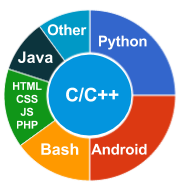
\includegraphics[scale=0.62]{img/programming.png}
    ~
  \section{OS Preference}
    \textbf{GNU/Linux}
\includegraphics[scale=0.40]{img/5stars.png}
    \textbf{Unix}
\includegraphics[scale=0.40]{img/4stars.png}
    \textbf{MacOS}
\includegraphics[scale=0.40]{img/3stars.png}
    \textbf{Windows}
\includegraphics[scale=0.40]{img/2stars.png}
    ~
  \section{Personal Skills}
    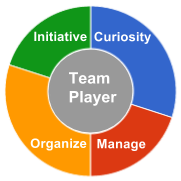
\includegraphics[scale=0.62]{img/personal.png}
    ~
 \section{agile Advocate}
 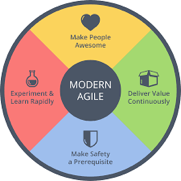
\includegraphics[scale=0.62]{img/agile.png}
\end{aside}

\section{Experience}
\begin{entrylist}
  \entry
    {02/17 - Now}
    {Senior Software Engineer}
    {Carmel, IN}
    {Responsible for feature work on hundreds of microservices. Created a modernized OCR pipeline, using AI deeplearning. Maintained a financial platform processing vehicle loans. Maintained high availability title management platform. Created cloud first solutions for application running in AWS. Assisted in the design and maturity of CI-CD solutions.  }
  \entry
    {01/18 - Now}
    {Freelance Developer \& Consultant}
    {Noblesville, IN}
    {High variance per customer ranging from WordPress CRM sites, to custom designed e-commerce solutions deployed to cloud infrastructure. }
    \entry
    {12/09 - 06/09}
    {Chart Biopsy LLC Software Engineer}
    {Indianapolis, IN}
    {Greenfield an entirely new EMR system. System needs to be compatible with data coming from EPIC EMR while maintaing PHI and PII compliance. }
    \entry
    {06/09 - 09/09}
    {Image Matters LLC (DoD Contractor, Software Engineer)}
    {Leesburg, VA}
    {Normalize, sort, and generate metadata using web-semantics and AI, for use by an ecosystem within the DoD. Systems were designed for highly-availability and efficient processing. }
    \entry
    {06/09 - 09/09}
    {Harmony Healthcare Software Engineer}
    {SouthBend, IN}
    {Primary developer responsible for the auto-matching of legacy medical databases, and emrs into newer medical systems. }
\end{entrylist}

\section{Education}
\begin{entrylist}
  \entry
    {2005 - 2009}
    {Bachelor's Degree in Software Engineering}
    {Indiana University}
    {Primary focus on algorithm design and functional programming \\
    \emph{Title of the Thesis: "Development, Management and Migrations of web contents and applications".}\\
    }
\end{entrylist}

\section{Certifications}
\begin{entrylist}
  \entry
    {02/2013}
    {Intro to Computer Science}
    {Udacity. E-learning}
    {\emph{Building a Python Search Engine}}
     \entry
    {02/2018}
    {Certified Solutions Architect – Associate }
    {AWS}
    {\emph{Effectively demonstrate knowledge of how to architect and deploy secure and robust applications on AWS technologies}}
\end{entrylist}
\section{Volunteer Work}
\begin{entrylist}
	\entry
	{02/2013}
	{Chip Indy}
	{}
	{\emph{Created a system for automating the availability of intimidate need resources for in-need minors.}}
	\entry
	{02/2018}
	{Certified Solutions Architect – Associate }
	{AWS}
	{\emph{Effectively demonstrate knowledge of how to architect and deploy secure and robust applications on AWS technologies}}
\end{entrylist}
\fcolorbox{white}{white}{\parbox{\dimexpr\textwidth-2\fboxsep-2\fboxrule}{}}
\fcolorbox{white}{white}{\parbox{\dimexpr\textwidth-2\fboxsep-2\fboxrule}{}}
\fcolorbox{white}{white}{\parbox{\dimexpr\textwidth-2\fboxsep-2\fboxrule}{}}
\fcolorbox{white}{white}{\parbox{\dimexpr\textwidth-2\fboxsep-2\fboxrule}{}}
\fcolorbox{white}{white}{\parbox{\dimexpr\textwidth-2\fboxsep-2\fboxrule}{}}
\end{document}
